% UPAR 2027 Track 1 paper, WACV 2026 author kit (the format required by the RWS workshop at WACV 2027).
\documentclass[10pt,twocolumn,letterpaper]{article}

%%%%%%%%% PAPER TYPE: \usepackage[review,algorithms]{wacv} for the anonymous review version
\usepackage{wacv}

%
% --- inline annotations
%
\newcommand{\red}[1]{{\color{red}#1}}
\newcommand{\todo}[1]{{\color{red}#1}}
\newcommand{\TODO}[1]{\textbf{\color{red}[TODO: #1]}}
% --- disable by uncommenting  
% \renewcommand{\TODO}[1]{}
% \renewcommand{\todo}[1]{#1}


\usepackage{booktabs}
\usepackage{multirow}
\usepackage{amsmath}
\usepackage{graphicx}
\graphicspath{{figs/}}

\definecolor{wacvblue}{rgb}{0.21,0.49,0.74}
\usepackage[pagebackref,breaklinks,colorlinks,allcolors=wacvblue]{hyperref}
\usepackage[capitalize]{cleveref}

\def\wacvPaperID{*****}
\def\confName{WACV}
\def\confYear{2027}
\newcommand{\pts}{\,pts}

\title{Fit Less to the Source: Complementary Encoders and a One-Parameter\\Decision Rule for Cross-Domain Pedestrian Attribute Recognition}

\author{Anonymous Authors\\
UPAR Challenge 2027, Track 1}

\begin{document}
\maketitle

%=====================================================================
\begin{abstract}
A pedestrian attribute recognizer deployed on a new camera loses accuracy in two ways. It ranks images worse than on its training cameras, and the decision thresholds it inherits from the source datasets no longer fit. Measured on held-out datasets, both losses are large, and they share a cause. Every quantity tuned on the source data, from the upper layers of a fine-tuned encoder to a per-attribute threshold, partly encodes the cameras and labelling conventions of those datasets. We therefore design a system that fits as little as possible to the source. Ranking comes from two foundation encoders of different pretraining families, DINOv3 ViT-H+ and CLIP ViT-L, fine-tuned only in their upper blocks, read by per-attribute query heads and averaged with fixed equal weights. Thresholds come from a decision rule with a single coefficient, whose target, balanced accuracy, does not depend on the label distribution of the new domain. We test each component against its source-fitted alternative. Fitted per-attribute thresholds and deeper fine-tuning both raise accuracy on the source domains, yet neither raises it reliably on held-out ones, whereas choosing the partner encoder by its held-out accuracy does. The system scores 0.7997 Challenge\_Avg on the hidden test set of UPAR 2027 Track~1.
\end{abstract}

%=====================================================================
\section{Introduction}
\label{sec:intro}

Searching surveillance footage for ``a woman in a pink top with a backpack'' needs a pedestrian attribute recognizer that works on cameras it has never seen. The usual PAR benchmarks~\cite{peta,pa100k,market} cannot measure this, because they draw training and test images from the same cameras. The UPAR challenges~\cite{upar,upar23,upar24} were created for this purpose. They train on several public datasets and test on a domain from which no training image comes.

When we evaluate our models in this way, by holding out one of the three training datasets, two kinds of error appear. The first is a ranking error. The mean AUC of a strong encoder falls by about four points from the training cameras to the held-out dataset, so the model orders images less correctly. The second is a threshold error. Even with the ranking unchanged, thresholds fitted on the held-out labels themselves would raise the challenge score by about three points, so the scores are also shifted. These two errors call for different remedies, and our system has one component for each.

What links the two components is the cause behind both errors. The source datasets differ from the target in their cameras and in how annotators named colors, lengths and accessories. Any parameter estimated on them absorbs some of these properties. This holds for the upper layers of a deeply fine-tuned encoder, for ensemble weights tuned on source validation data and for per-attribute thresholds. Such parameters improve the source domains, but their improvement need not carry over. We therefore follow one principle throughout. The system should fit as little as possible to the source and obtain its accuracy from components that do not depend on it.

The principle shapes every part of the system. The diversity of the ensemble comes from pretraining rather than fine-tuning. We combine a self-supervised DINOv3 ViT-H+~\cite{dinov3} and an image-text CLIP ViT-L~\cite{clip}, whose errors differ because their pretraining differs, and fine-tune both only in their upper blocks. Their logits are averaged with fixed equal weights, and the thresholds come from a logit adjustment with one coefficient instead of forty fitted offsets. Our contributions are:
\begin{itemize}
\item A measurement of the ranking and threshold errors on held-out datasets, and the principle it suggests (\cref{sec:loss}).
\item A system derived from this principle, built from complementary encoders with query heads, an equal-weight ensemble and a one-parameter decision rule (\cref{sec:method}).
\item Tests of each component against its source-fitted alternative, which show that gains on the source domains do not predict gains on held-out ones, confirmed on the hidden test set (\cref{sec:experiments}).
\end{itemize}

%=====================================================================
\section{Related Work}
\label{sec:related}

\paragraph{Pedestrian attribute recognition.} DeepMAR~\cite{deepmar} framed PAR as multi-label classification with a loss weighted by attribute frequency, a weighting still widely used. Later methods added modules that localize attributes or model their relations, but Jia~\etal~\cite{rethinkpar} showed that many of these gains disappear under a stricter split. Much reported progress may therefore have come from fitting the evaluation data more closely. Query-based heads~\cite{q2l,mldecoder}, which we adopt, give each label its own query over the image tokens. UPAR~\cite{upar} unified four datasets into 40 attributes and made cross-domain evaluation possible.

\paragraph{Generalization with pretrained encoders.} With a strong backbone, plain empirical risk minimization matches specialized domain generalization methods~\cite{domainbed}. Fine-tuning, however, can distort pretrained features and hurt out-of-distribution accuracy~\cite{lpft}, which motivates partial fine-tuning and weight interpolation~\cite{wiseft}. Weight averaging of several fine-tuned models~\cite{soups,diwa} adds robustness at no inference cost but requires a shared initialization. These works ask how far an encoder should move away from pretraining. We ask the same question for every source-fitted component of a PAR system.

\paragraph{Ensembles under distribution shift.} The error of an ensemble falls with the accuracy of its members and with their disagreement~\cite{krogh}, and deep ensembles remain among the most reliable predictors under dataset shift~\cite{deepens,ovadia}. To our knowledge, it has not been measured which of the two factors matters when the members are fine-tuned foundation encoders and the metric is thresholded.

\paragraph{Label shift and logit adjustment.} When class priors change, posteriors can be corrected by the ratio of priors~\cite{saerens,lipton}, and adding a scaled log prior to the logits optimizes balanced error~\cite{logitadj}. Our decision rule is this adjustment with one extra term that removes the shift already introduced by the DeepMAR loss weights.

%=====================================================================
\section{Setting}
\label{sec:setting}

\paragraph{Task and metric.} Each pedestrian crop has 40 binary attributes, covering age (three classes), gender, hair length (three classes), sleeve length, lower-body length and type, twelve upper-body and twelve lower-body clothing colors, and five accessories. The training data are the UPAR re-annotations of PA100k, Market1501 and PETA (\cref{tab:data}), and the hidden test set holds 29{,}248 images from a fourth domain. The challenge score Challenge\_Avg (Avg) is the harmonic mean of two quantities. The first, mA, is the balanced accuracy averaged over attributes. The second, instance F1, is the F1 score of each image's predicted attribute set, averaged over images. Both use a fixed threshold of 0.5. We report scores $\times100$ and differences in points (pts).

\begin{table}[t]
\centering\small
\setlength{\tabcolsep}{3pt}
\resizebox{\columnwidth}{!}{%
\begin{tabular}{@{}lrrl@{}}
\toprule
Dataset & Train & Val & Images \\
\midrule
PA100k~\cite{pa100k} & 79{,}001 & 9{,}986 & outdoor, about 600 cameras \\
Market1501~\cite{market,marketattr} & 10{,}000 & 16{,}458 & one campus, $128\times64$ crops \\
PETA~\cite{peta} & 8{,}668 & 6{,}963 & ten pooled sources \\
\bottomrule
\end{tabular}}
\caption{Training data of UPAR 2027 Track~1.}
\label{tab:data}
\end{table}

\paragraph{Held-out protocol.} Because the target domain is unseen, we evaluate design choices on a domain the model has not seen either. We train on the training splits of two datasets and score the validation split of the third. PETA, whose ten pooled sources make it the most varied, is the main held-out domain, and Market1501 serves as a second one for the key comparisons. For the PETA-held-out models, the validation images of Market1501 and PA100k give an in-domain score on images that were not used in training. Comparing the in-domain and the held-out effect of the same change is the central measurement of this paper. Protocol models are trained for three epochs on two datasets, and the submitted models for three epochs on the training and validation splits of all three.

\paragraph{Noise.} Four runs of CLIP ViT-L/14 with the same recipe, differing only in seed, machine or activation implementation, score between 81.13 and 81.58 on held-out PETA. Paired with the same DINOv3 model, they score between 82.17 and 82.42. We therefore treat differences below about 0.3\pts{} between single runs as unreliable.

%=====================================================================
\section{Where Accuracy Is Lost}
\label{sec:loss}

Before designing the system, we measure how large the two errors are. We use the encoder pair of \cref{sec:method} with all thresholds at 0.5, so that the decision rule plays no part yet. Its ranking quality, measured by mean AUC, is 96.71 on the in-domain images and 92.97 on held-out PETA. A substantial part of the loss therefore comes from ordering images worse on the new domain.

The threshold error is measured with an oracle. We fit one offset per attribute on the held-out labels themselves and add it to the logits. This oracle cannot be used at test time, but its gain over the plain threshold bounds what any threshold rule could achieve on that domain. It gains 3.09\pts{} of Avg on PETA and 2.54\pts{} on Market1501. In earlier experiments on the same protocol we traced most of this gap to clothing colors, whose labelling differs between datasets. PETA, for instance, assigns two colors to 12\% of upper garments, whereas the other datasets almost never do.

The two measurements point to one cause. A model fine-tuned on the source datasets learns their cameras and conventions, so it ranks worse on a new domain. Thresholds fitted on the source datasets learn the same conventions, so they land in the wrong place. Fitting the source more closely cannot remove either error and may increase both. This is the principle behind the method that follows. Accuracy should come from components that do not depend on the source domains, and every source-fitted component should be kept as small as possible.

%=====================================================================
\section{Method}
\label{sec:method}

\subsection{Complementary encoders, conservatively fine-tuned}
\label{sec:encoders}

The ranking component has to order attributes correctly under changes of resolution, viewpoint, color rendering and labelling style. Foundation encoders pretrained on large and varied image collections offer features that are robust to such changes, which leaves two requirements. The features must stay close to pretraining, and the errors of the system must not all be of one kind, since a single encoder errs systematically on a new domain.

We meet the first requirement by fine-tuning only the upper blocks. The patch embedding and the first eight transformer blocks are frozen, and the remaining blocks are trained with layer-wise learning-rate decay~\cite{beit}. Block $l$ of $L$ receives the learning rate $\eta\,\gamma^{L-l}$ with $\gamma=0.75$, which concentrates the effective update in the top blocks. We meet the second requirement with two encoders whose pretraining differs in both data and objective. DINOv3 ViT-H+/16~\cite{dinov3} is trained by self-distillation on images alone, while CLIP ViT-L/14~\cite{clip} is trained to match images with captions. Both read a $224\times112$ crop, which DINOv3 divides into $14\times7$ patch tokens and CLIP into $16\times8$. In this design the diversity of the ensemble comes from pretraining, which is fixed, rather than from fine-tuning, which would fit the source.

\paragraph{Query head.} Different attributes depend on different regions, such as the face for glasses and the legs for a skirt, so a head that pools all tokens into one vector mixes their evidence. We therefore use a query head~\cite{q2l,mldecoder}. Each attribute $k$ owns a learned query $q_k$ that attends to the token matrix $X$ of the encoder, formed by the class token and the patch tokens,
\begin{align}
h_k &= q_k + \mathrm{MHA}\big(\mathrm{LN}(q_k),\,\mathrm{LN}(X)\big),\\
z_k &= w_k^{\top}\,\mathrm{LN}\big(h_k + \mathrm{MLP}(\mathrm{LN}(h_k))\big) + c_k .
\end{align}
In the first line, multi-head attention (MHA, eight heads) lets query $k$ gather the tokens relevant to its attribute. In the second line, a small MLP refines the result, and a classifier $(w_k,c_k)$ that belongs to attribute $k$ alone maps it to the logit $z_k$. \Cref{fig:method} shows that the queries settle on the regions their attributes describe, even on a dataset that neither encoder saw during training.

\paragraph{Training objective.} The loss is binary cross-entropy with label smoothing $\epsilon=0.05$ and the DeepMAR weights~\cite{deepmar} $w_k^{+}=e^{1-\pi_k}$ for positives and $w_k^{-}=e^{\pi_k}$ for negatives, where $\pi_k$ is the training prior of attribute $k$. The weights counter the rarity of most attributes, and the decision rule of \cref{sec:rule} removes the shift they introduce. Datasets are sampled in proportion to $N_d^{0.5}$, so that PA100k, eight times larger than the others, does not dominate training. The remaining details are in \cref{app:config}.

\begin{figure*}[t]
\centering
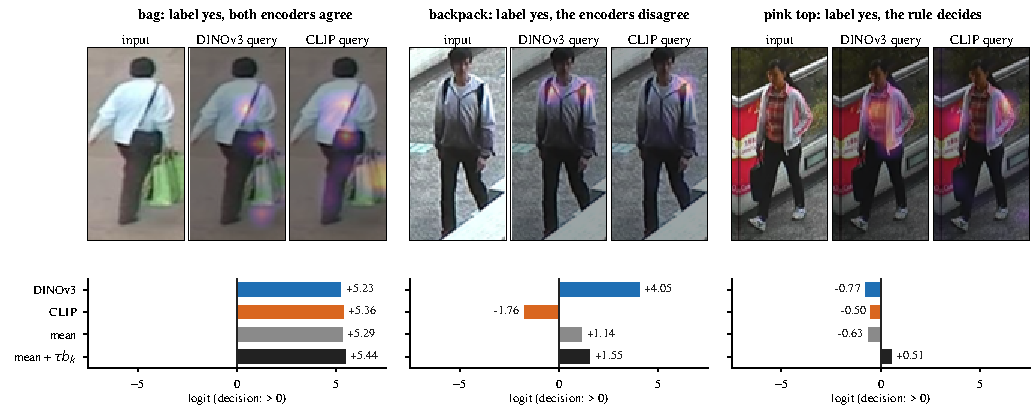
\includegraphics[width=\linewidth]{method_cases.pdf}
\caption{The method on three PETA images, for an encoder pair that never saw PETA. Top: input and the attention of each encoder's query for the named attribute. Bottom: the logit of each encoder, their mean, and the mean after the decision rule.}
\label{fig:method}
\end{figure*}

\subsection{Equal-weight logit averaging}
\label{sec:ensemble}

The two encoders each produce one logit per attribute, and we average them with equal weights, $\bar z_k=\tfrac12(z_k^{\text{DINO}}+z_k^{\text{CLIP}})$. Averaging logits rather than probabilities lets a confident member outweigh an uncertain one. In the backpack example of \cref{fig:method}, DINOv3 is confidently right and CLIP is wrong with less confidence, so the mean follows DINOv3. Weights tuned on source validation data would be one more fitted parameter, and the weight that suits one domain need not suit another. Equal weights avoid this choice, and \cref{sec:design} measures what they cost.

\subsection{One-parameter decision rule}
\label{sec:rule}

The mean logit must finally be compared with the threshold of 0.5. The usual remedy for misplaced thresholds is a per-attribute offset fitted on source validation data. As \cref{sec:loss} showed, however, such offsets learn the conventions of the source datasets. They are also noisy, because many attributes have few positives. A rule for an unseen domain should instead have few parameters, and its target should not depend on the label distribution of that domain.

The mA half of the metric supplies such a target. Balanced accuracy weighs positives and negatives equally, so its optimal decision is the one made under a balanced prior, whatever the true prior of the target domain is. If the model is calibrated under the training prior $\pi_k$, moving to a balanced prior adds $\log\frac{1-\pi_k}{\pi_k}$ to the logit~\cite{saerens,logitadj}. The DeepMAR weights have already moved the optimum of the training loss by $\log(w_k^{+}/w_k^{-})=1-2\pi_k$ in the same direction, so only the difference remains to be added,
\begin{equation}
b_k=\log\frac{1-\pi_k}{\pi_k}-(1-2\pi_k),\qquad z_k \leftarrow \bar z_k+\tau\,b_k .
\label{eq:rule}
\end{equation}
Instance F1, the other half of the metric, prefers fewer positives for rare attributes. A single coefficient $\tau\in[0,1]$ trades the two halves off, from the decision of the weighted loss at $\tau=0$ to the mA-optimal decision at $\tau=1$. For a rare attribute such as a pink top ($\pi_k\approx0.02$), $b_k$ is large and positive, which is why the rule turns the correct but negative mean logit of the third example in \cref{fig:method} into a positive decision. For a frequent attribute such as trousers ($\pi_k\approx0.9$), $b_k$ is negative. We use $\tau=0.42$, a value set in earlier single-model experiments on the PETA-held-out protocol, with priors from all training and validation labels. Because the derivation ignores label smoothing and assumes calibration under $\pi_k$, it fixes the form of the rule rather than the value of $\tau$.

%=====================================================================
\section{Experiments}
\label{sec:experiments}

The method rests on two claims. Components fitted to the source should not be trusted on a new domain, and accuracy should come from what does not depend on the source. \Cref{sec:fitting} tests the first claim directly. \Cref{sec:pairing,sec:design} then examine how the ensemble was built, \cref{sec:rule_exp} the decision rule, and \cref{sec:test} the hidden test.

\subsection{Source-fitted alternatives}
\label{sec:fitting}

\Cref{tab:fitting} replaces each component of the system by an alternative fitted more closely to the source and reports the change on the in-domain images and on the held-out domains. The pattern is consistent. Every alternative raises the in-domain score, where it is fitted, while its effect on held-out domains is either negative or within the noise band.

Per-attribute offsets fitted on the in-domain validation data show the pattern most clearly. They raise the in-domain score of the ensemble, although that figure is optimistic because it is measured on the data used for fitting. On held-out PETA, the same offsets fall below the one-parameter rule by about as much. Deeper fine-tuning, with four frozen blocks and $\gamma=0.9$, gives the middle blocks of ViT-H+ about twenty times larger learning rates. It raises the in-domain score of every encoder. On held-out data it helps DINOv3, hurts CLIP on PETA and moves the ensemble only within the noise band, and \cref{sec:test} shows that it loses on the hidden test. The member weight is the one fitted quantity that does no harm. The weight that is best in-domain is almost exactly the equal weight we use, so tuning it neither helps nor hurts.

\begin{table}[t]
\centering\small
\setlength{\tabcolsep}{3pt}
\resizebox{\columnwidth}{!}{%
\begin{tabular}{@{}llccc@{}}
\toprule
Our choice & Source-fitted alternative & in-domain & PETA & Market1501 \\
\midrule
one-parameter rule & fitted per-attribute offsets & +0.55 & $-$0.53 & -- \\
conservative fine-tuning & deeper, DINOv3-H+ alone & +0.51 & +0.59 & +0.18 \\
conservative fine-tuning & deeper, CLIP-L alone & +0.44 & $-$0.44 & +0.03 \\
conservative fine-tuning & deeper DINOv3 in the ensemble & +0.21 & +0.18 & +0.07 \\
equal weights & best in-domain weight (0.6) & +0.01 & $-$0.04 & +0.11 \\
\bottomrule
\end{tabular}}
\caption{Change in Avg when a component is replaced by an alternative fitted more closely to the source domains.}
\label{tab:fitting}
\end{table}

\subsection{Choosing the partner encoder}
\label{sec:pairing}

If accuracy is to come from pretraining, the choice of the second encoder is the most important decision. We fine-tuned ten foundation encoders with the recipe of \cref{sec:encoders} and paired each with DINOv3 ViT-H+ (\cref{tab:encoders}). CLIP ViT-L/14 is the best partner on both readouts, followed by the closely related MetaCLIP ViT-L/14~\cite{metaclip}.

The table also shows what makes a partner good, and ranking quality alone does not. Both SigLIP2 encoders~\cite{siglip2} rank PETA about as well as CLIP, with a similar AUC, yet they form two of the four weakest pairs. Across the nine partners, the partner's own held-out Avg predicts the pair's Avg with a Spearman correlation of 0.92, whereas its AUC reaches only 0.42. The SigLIP2 encoders produce more false positives than CLIP on rare attributes such as glasses, old age and baldness, and averaging with DINOv3 does not remove them. Because the metric is thresholded, a partner helps through correct decisions and not only through a correct ordering, so it should be chosen by its held-out accuracy.

\begin{table}[t]
\centering\small
\setlength{\tabcolsep}{2.6pt}
\resizebox{\columnwidth}{!}{%
\begin{tabular}{@{}llccccc@{}}
\toprule
& & \multicolumn{3}{c}{single encoder} & \multicolumn{2}{c}{with DINOv3-H+} \\
\cmidrule(lr){3-5}\cmidrule(l){6-7}
Encoder & Input & PETA & AUC & in-dom. & PETA & in-dom. \\
\midrule
DINOv3 ViT-H+/16~\cite{dinov3} & 224$\times$112 & 81.42 & 92.23 & 88.66 & -- & -- \\
\midrule
CLIP ViT-L/14~\cite{clip} & 224$\times$112 & 81.54 & 91.87 & 88.38 & 82.33 & 89.14 \\
MetaCLIP ViT-L/14~\cite{metaclip} & 224$\times$112 & 81.35 & 92.04 & 88.51 & 82.14 & 89.19 \\
EVA02-CLIP ViT-L/14~\cite{evaclip} & 224$\times$112 & 80.58 & 90.97 & 87.94 & 82.03 & 89.02 \\
AIMv2 ViT-L/14~\cite{aimv2} & 224$\times$112 & 80.23 & 91.40 & 87.82 & 81.90 & 88.96 \\
PE-Core ViT-L/14~\cite{pe} & 224$\times$112 & 80.71 & 91.23 & 88.06 & 81.88 & 89.02 \\
MetaCLIP2 ViT-H/14~\cite{metaclip2} & 168$\times$84 & 80.42 & 91.63 & 87.29 & 81.87 & 88.84 \\
SigLIP2 So400m/14~\cite{siglip2} & 224$\times$112 & 80.12 & 91.67 & 87.60 & 81.86 & 88.94 \\
SigLIP2 ViT-L/16~\cite{siglip2} & 256$\times$128 & 80.12 & 91.76 & 87.81 & 81.68 & 89.01 \\
DFN-CLIP ViT-L/14~\cite{dfn} & 224$\times$112 & 79.37 & 90.87 & 86.95 & 81.63 & 88.78 \\
\bottomrule
\end{tabular}}
\caption{Encoders alone and paired with DINOv3 ViT-H+ by logit averaging, with PETA held out during training.}
\label{tab:encoders}
\end{table}

\subsection{Combining the pair}
\label{sec:design}

With the partner chosen, three questions remain. Should the pair be weighted, extended or compressed into one model (\cref{tab:design})? The best member weight differs between domains. On PETA it is the equal weight, while on Market1501 it moves towards DINOv3, which alone is as good as any mixture there. Equal weights stay within 0.11\pts{} of the best weight on both domains, whereas relying on one encoder loses up to 0.91\pts{} on one of them. Without knowledge of the target domain, equal weights are the safe choice.

Extending the pair with a third member does not help. None of four candidates improves the pair, including MetaCLIP2 ViT-H/14, the largest encoder we tried. A third member is mostly similar to one already present, and on a thresholded metric its false positives weigh as much as its corrections.

Compressing the pair loses accuracy. We distilled an ensemble of DINOv3 ViT-H+, CLIP ViT-L/14 and MetaCLIP2 ViT-H/14 into one DINOv3 ViT-H+ student, using soft targets~\cite{hinton} on mixed inputs for 15 epochs. The student alone is as accurate as the best single encoder of this study. Paired with CLIP, however, it gains less than the original DINOv3 model does, because it has absorbed CLIP's predictions and no longer disagrees with it. The pairing gain thus depends on members trained independently, which is what the equal-weight ensemble of \cref{sec:ensemble} provides.

\begin{table}[t]
\centering\small
\setlength{\tabcolsep}{4pt}
\begin{tabular}{@{}lcc@{}}
\toprule
Variant & PETA & Market1501 \\
\midrule
DINOv3-H+ + CLIP-L, equal weights & 82.33 & 86.35 \\
\quad weight of DINOv3-H+ 0.4 & 82.30 & 86.23 \\
\quad weight of DINOv3-H+ 0.6 & 82.29 & 86.46 \\
\quad DINOv3-H+ alone & 81.42 & 86.46 \\
\quad CLIP-L alone & 81.54 & 85.60 \\
\midrule
+ MetaCLIP ViT-L/14 & 82.32 & -- \\
+ MetaCLIP2 ViT-H/14 & 82.27 & -- \\
+ AIMv2 ViT-L/14 & 82.16 & -- \\
+ SigLIP2 So400m/14 & 82.15 & -- \\
\midrule
distilled DINOv3-H+ student alone & 82.00 & -- \\
distilled student + CLIP-L & 82.21 & -- \\
\bottomrule
\end{tabular}
\caption{Weighting, extending and compressing the pair, with each domain held out during training.}
\label{tab:design}
\end{table}

\subsection{The decision rule}
\label{sec:rule_exp}

\Cref{sec:fitting} showed that the one-parameter rule transfers better than fitted offsets. \Cref{fig:tau} shows how much it recovers and how sensitive it is to its single parameter. On PETA the rule raises the ensemble by 1.24\pts{} over the plain threshold, and on Market1501 by 0.84\pts. The single encoders gain by similar amounts, so the rule and the ensemble correct different parts of the error and their gains add up. All curves rise until $\tau$ reaches 0.5 to 0.65 and collapse soon after, when rare attributes are predicted far too often and instance F1 breaks down. The value $\tau=0.42$, chosen before these models existed, lies on the rising part on both domains, close to the best value and away from the collapse.

Measured against the oracle of \cref{sec:loss}, the rule closes about 40\% of the threshold gap on PETA and a third of it on Market1501. The remaining 1.85\pts{} and 1.70\pts{} exceed every difference between encoders in \cref{tab:encoders}. This remainder is the part of the error that depends on the conventions of the target domain, and no rule estimated from the source can recover it.

\begin{figure}[t]
\centering
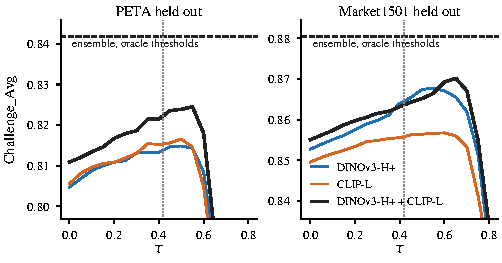
\includegraphics[width=\linewidth]{tau_rule.pdf}
\caption{Challenge\_Avg as a function of the decision-rule coefficient $\tau$ on two held-out domains. The dotted line marks the submitted value and the dashed line the ensemble with oracle thresholds.}
\label{fig:tau}
\end{figure}

\subsection{Hidden-test results}
\label{sec:test}

The hidden test is the final check of the protocol and of the principle. \Cref{tab:test} lists our main submissions with the PETA-held-out score of each recipe. The protocol orders the first three submissions as the test does. Moving from a single distilled DINOv3 ViT-L to an ensemble of four models gains 0.63\pts{} on the test set. Replacing that ensemble by the DINOv3 ViT-H+ and CLIP ViT-L pair, which is smaller and better on the protocol, adds 0.22\pts. The protocol score of v20 uses the ten-epoch student of v13 in place of its longer-trained student. The fourth submission is the deeper fine-tuning of \cref{sec:fitting}. Its protocol gain lies inside the noise band, and on the test it loses 0.10\pts, as \cref{tab:fitting} anticipates for a source-fitted change. The submitted system v21 reaches an mA of 80.61 and an instance F1 of 79.33 on the test set, with precision 75.61 and recall 84.90.

\begin{table}[t]
\centering\small
\setlength{\tabcolsep}{3pt}
\resizebox{\columnwidth}{!}{%
\begin{tabular}{@{}llcc@{}}
\toprule
& Members & PETA held out & Hidden test \\
\midrule
v13 & distilled DINOv3 ViT-L/16 student & 81.18 & 79.12 \\
v20 & student + DINOv3 ViT-L + CLIP-L + MetaCLIP2-H & 82.03 & 79.75 \\
v21 & DINOv3 ViT-H+ + CLIP ViT-L (this paper) & 82.33 & 79.97 \\
v22 & v21 with deeper DINOv3 fine-tuning & 82.51 & 79.87 \\
\bottomrule
\end{tabular}}
\caption{Submissions to UPAR 2027 Track~1 and the protocol scores of their recipes.}
\label{tab:test}
\end{table}

%=====================================================================
\section{Conclusion}
\label{sec:conclusion}

On a new camera, a pedestrian attribute recognizer loses accuracy through ranking and through thresholds, and both losses arise because parameters fitted on the source datasets encode those datasets. Designing against this cause leads to a simple system. Two encoders from different pretraining families are fine-tuned only in their upper blocks and averaged with equal weights, and a single coefficient sets all thresholds. Each source-fitted alternative we tested improved the source domains without a reliable gain on held-out ones. The largest remaining error lies in the labelling conventions of the target domain, which no component fitted on the source can learn.

\paragraph{Limitations.} Most comparisons rest on one held-out dataset and one training run per configuration, and the noise estimate comes from one encoder. \Cref{fig:method} uses the ViT-L members of an earlier ensemble of the same two families, trained with the same recipe, because the held-out version of the submitted ViT-H+ model was not kept. The decision rule assumes priors estimated from representative training data.

\paragraph{Broader impact.} Attribute recognition on surveillance video, including age and gender, can support tracking of individuals. We report technical findings only and do not release models trained on surveillance data.

{\small
\bibliographystyle{ieeenat_fullname}
\bibliography{refs}
}

%=====================================================================
\clearpage
\appendix
\section{Training configuration}
\label{app:config}

Both encoders use the same recipe. The optimizer is AdamW with learning rate $5\cdot10^{-5}$ at the last block, layer decay $\gamma=0.75$, a head learning rate ten times larger, weight decay 0.05 and batch size 64. The schedule is cosine with half an epoch of warm-up and lasts three epochs. Training uses stochastic depth 0.1, bf16 mixed precision and an exponential moving average of the weights with decay 0.9995, which is the model used at test time. The query head has one layer, eight attention heads, an MLP ratio of two and dropout 0.1. Augmentation consists of random down-scaling to simulate low-resolution crops, horizontal flip, edge padding of ten pixels followed by a random crop, brightness, contrast and saturation jitter without hue change, Gaussian blur and random erasing. Priors $\pi_k$ are clipped to $[10^{-3},1-10^{-3}]$, and cells that a dataset does not annotate are masked in the loss. The two submitted members are trained on the training and validation splits of all three datasets. At test time both read the same crop resized to $224\times112$, and the pair processes the 29{,}248 test images in about four minutes on one NVIDIA A10 GPU.

\end{document}
